\documentclass[11pt]{article}

\usepackage[T1]{fontenc}
\usepackage[utf8]{inputenc}
\usepackage{lmodern}
\usepackage{amsmath,amssymb}
\usepackage[letterpaper,margin=1in]{geometry}
\usepackage{booktabs}
\usepackage{tabularx}
\usepackage{array}
\usepackage{graphicx}
\usepackage{hyperref}

\hypersetup{colorlinks=true,linkcolor=blue,citecolor=blue,urlcolor=blue}
\setlength{\emergencystretch}{3em}
\newcolumntype{Y}{>{\raggedright\arraybackslash}X}

\title{Spectral Covariance Cleaning, Portfolio Breadth, and Market Proxies:\\
Evidence from Mexican Equities}
\author{Julio C\'esar Galindo L\'opez\\
\small Universidad Panamericana, Ciudad UP
\and
Laura Jim\'enez Casillas\\
\small Universidad Panamericana, Ciudad UP}
\date{Working paper --- 30 September 2026}

\begin{document}
\maketitle

\begin{abstract}
Does nonlinear RMT covariance cleaning reduce out-of-sample minimum-variance
portfolio risk without diminishing allocation breadth in Mexican equities,
and how does the observed relationship vary across market proxies and
asset-to-observation ratios? We compare sample, eigenvalue-clipped,
Ledoit--Wolf, and
rotationally invariant (RIE) covariance estimators on a common, chronological
holdout from a 38-stock Bolsa Mexicana de Valores panel. On 529 test days, daily
realized volatility is 0.6794\% per day for RIE and 0.6884\% for the sample
estimator, a 1.31\% relative difference. This volatility comparison is
descriptive: the paired 20-day moving-block bootstrap for the annualized
Sharpe difference is $+0.011$ (95\% interval $[-0.021,0.057]$; one-sided
$p=0.186$). RIE's inverse-Herfindahl effective holdings count is 9.86 versus
9.36, while Shannon effective breadth is 26.92 for both; allocation-breadth
conclusions depend on the measure. Two provisional VOM-labelled Bloomberg
proxies show higher conditional holdout volatility above training-period
90th-percentile thresholds, but their economic definitions are undocumented
and the comparisons are descriptive. In a recent 25-stock, 100-return panel
($q=0.25$), eigenvalue clipping reduces the correlation condition number from
24.34 to 5.33. In ten deliberately short $q=1.9$ windows, this RIE
implementation is unstable, with 144.43\% mean annualized realized
volatility. The evidence supports a conditional, limited case for spectral
regularization, not universal estimator dominance or a market-wide claim about
investor diversity.
\end{abstract}

\noindent\textbf{Keywords:} random matrix theory; covariance estimation; Mexican
equity market; minimum-variance portfolio; covariance conditioning; portfolio
concentration; out-of-sample evaluation.

\section{Introduction}

The sample covariance matrix is a noisy input to portfolio optimization when
the number of assets is not negligible relative to the return-history length.
Because minimum-variance weights depend on its inverse, errors in the smallest
sample eigenvalues can be magnified in the resulting positions. Random matrix
theory (RMT) provides principled spectral corrections, including nonlinear
shrinkage estimators that preserve the sample eigenvectors while modifying
eigenvalues \cite{markowitz1952,demiguel2009,marchenko1967,laloux1999,ledoit2022}.
Early empirical work
documented noise in financial correlation spectra, while subsequent studies
connected cleaning to portfolio optimization
\cite{pafka2002,ledoitwolf2004}. Whether these corrections remain useful
across market conditions while maintaining broad allocations is an empirical
question for emerging equity markets.

\paragraph{Research question.}
\emph{Does nonlinear RMT spectral covariance cleaning lower out-of-sample
minimum-variance portfolio risk without reducing allocation breadth in
Mexican equities, and how do the observed risk and breadth outcomes vary with
market proxies and the asset-to-observation ratio $q=N/T$?}

The article answers this question with one common chronological holdout for
the primary estimator comparison, two separately exported Bloomberg
market-indicator series for descriptive conditioning, and a recent
high-dimensional cross-section. Each supplementary dataset has a distinct
role; none is pooled into the primary panel.

The contribution is deliberately empirical and bounded: (i) a common-date
comparison separates small realized-volatility differences from Sharpe-ratio
uncertainty; (ii) two distinct allocation-breadth measures reveal that a
diversity conclusion is metric-dependent; and (iii) high-dimensional checks
document improved conditioning at $q=0.25$ but instability of this particular
unmodified RIE implementation at $q=1.9$.

\section{Data and methods}

\subsection{Primary BMV panel}

The primary panel comprises 38 Mexican equities and 2,644 daily log-return
observations, from 18 July 2011 through 29 September 2025, derived from adjusted
Econom\'atica prices. The tickers are MFRISCOA-1, RA, SIMECB, FUNO11, ICHB,
GENTERA, SORIANAB, ELEKTRA, CHDRAUIB, LIVEPOLC-1, AUTLANB, HERDEZ, GAPB,
OMAB, MEGACPO, PINFRA, LABB, ALSEA, ARA, ASURB, AMXB, AC, AXTELCPO,
KIMBERA, CEMEXCPO, BIMBOA, BOLSAA, GCARSOA1, FEMSAUBD, GFNORTEO, GFINBURO,
ORBIA, GRUMAB, GMEXICOB, PE\&OLES, TLEVISACPO, SIGMAFA, and WALMEX. We
reserve the final 529 observations (3 May 2021--29
September 2025) as a chronological holdout and estimate the covariance matrix
on the preceding 2,115 observations. Thus $q=N/T_{\mathrm{train}}=38/2115
\approx0.0180$. This common split is used for the estimator comparisons in
Sections~\ref{sec:holdout}--\ref{sec:factor}; it avoids mixing results computed
on different test windows.

Daily log returns are computed from adjusted prices. We compare the sample
covariance (SM), Mar\v cenko--Pastur eigenvalue clipping (CL), Ledoit--Wolf
linear shrinkage (LW), and analytic nonlinear rotationally-invariant
shrinkage (RIE). CL standardizes to a correlation matrix, retains sample
eigenvalues above the Mar\v cenko--Pastur upper edge, replaces the remaining
bulk eigenvalues by their average, and restores the original marginal scales.
For sample aspect ratio $q=N/T<1$, the theoretical noise support is
$[\lambda_-,\lambda_+]$ with
$\lambda_{\pm}=(1\pm\sqrt{q})^2$ under the Mar\v cenko--Pastur benchmark.
LW is the standard identity-target linear shrinkage estimator. RIE applies
kernel-based analytic nonlinear shrinkage to the sample eigenvalues while
retaining the sample eigenvectors. The RIE implementation is designed for
$q<1$; this article does not claim that the implementation is valid for
$q\geq1$.

For each estimate $\widehat\Sigma$, the unconstrained global minimum-variance
weights are
\[
  \widehat w =
  \frac{\widehat\Sigma^{-1}\mathbf{1}}
       {\mathbf{1}^{\mathsf T}\widehat\Sigma^{-1}\mathbf{1}},
  \qquad \mathbf{1}^{\mathsf T}\widehat w=1.
\]
All four methods use the same training dates, test dates, return units, and
fully invested constraint. The covariance estimates and weights are fit once
on the training sample and held fixed through the full chronological test
window; this is a static holdout comparison, not a rolling rebalancing
strategy. We do not include transaction costs, turnover, liquidity limits,
market impact, short-sale constraints, or leverage constraints.

The primary outcomes are annualized Sharpe ratio (using an assumed 8\% annual
risk-free rate), realized daily volatility on the holdout, and two
allocation-breadth measures. The assumed risk-free rate is fixed across all
estimators; results under alternative risk-free rates are not reported. The
inverse-Herfindahl effective holdings count is
$\mathrm{NEA}=1/\sum_i w_i^2$. Shannon breadth is
$\exp(H)$, where
$H=-\sum_i p_i\log p_i$ and
$p_i=|w_i|/\sum_j|w_j|$; absolute weights are used because the unconstrained
portfolios may contain short positions. With short positions, neither metric
should be read literally as a count of positive holdings: both are
portfolio-level summaries and say nothing about the diversity of market
participants.

For a portfolio return $r_{p,t}$, the annualized Sharpe is computed as
$\sqrt{252}\,(\bar r_p-r_f/252)/s_p$, with daily sample standard deviation
$s_p$. The risk comparison is reported in percent per trading day. The primary
Sharpe-difference interval is estimated by a paired moving-block bootstrap
with 5,000 replications and 20-day blocks, using the same resampled date
indices for both portfolios. The reported one-sided $p$-value tests whether
the Sharpe difference is non-positive; no corresponding confidence interval
for the volatility difference is available. Accordingly, the volatility gap
is descriptive and is not presented as an inferentially established effect.

\subsection{Supplementary market data and sample construction}

Table~\ref{tab:sources} records the datasets used. The primary 38-stock panel
supports the estimator comparison. A separate Bloomberg export supplies two
VOM-labelled daily series, the NAFTRAC field \texttt{PR093}, and the
USD/MXN exchange rate. A second Bloomberg workbook supplies daily fields for
a recent 25-stock cross-section. These supplementary samples are used for
descriptive regime conditioning and an aspect-ratio boundary check,
respectively; they are not pooled with the primary return panel.

\begin{table}[ht]
\centering
\caption{Available data and role in the analysis.}
\label{tab:sources}
\small
\begin{tabularx}{\textwidth}{>{\raggedright\arraybackslash}p{3.1cm}>{\raggedright\arraybackslash}p{4.1cm}>{\raggedright\arraybackslash}p{2.5cm}Y}
\toprule
Source & Observed material & Availability & Role here \\
\midrule
BMV--Econom\'atica & 38 equities; 2,644 daily returns, 2011--2025 &
Derived panel; raw licensed prices not redistributable &
Primary common holdout and estimator comparison; universe selection may
induce survivorship or selection bias \\
Bloomberg VOM/FX export & Two VOM-labelled series, NAFTRAC
\texttt{PR093}, USD/MXN; 2000--2026 & Daily CSV export; some dates absent &
Convert VOM levels to MXN and condition holdout risks on training-period
thresholds \\
Bloomberg BMV/BIVA workbook & 275 instrument tabs and daily fields; 2000--2026 &
Licensed XLSX export &
Recompute the matched $N=25$, $T=100$, $q=0.25$ check using gross total returns \\
Fama--French 5 factors & Daily U.S. factors, matched to BMV dates &
Public factor file & Secondary pricing-model check \\
\bottomrule
\end{tabularx}
\end{table}

\paragraph{Currency treatment and VOM-regime construction.}
The Bloomberg export identifies \texttt{VOMXCUS\$ Index} and
\texttt{VOMXGUS\$ Index} as USD-denominated series and includes daily
\texttt{MXN BGN Curncy}. Following the export note, we convert each observed
VOM level to pesos by multiplying by the same-date USD/MXN rate. We use no
cross-series comparison of raw levels: in particular, NAFTRAC's exported field
is \texttt{PR093}, not a closing price, so it is not treated as a return or
compared numerically with either VOM series. For each VOM series separately,
the high-state threshold is its 90th percentile in the primary training period
(18 July 2011--30 April 2021), and this fixed threshold is applied to matched
holdout dates. There are 506 matched days (out of 529); the final VOM data
date is 17 September 2025. The CSV does not include a Bloomberg field
description for the VOM tickers; their interpretation as market-stress
indicators is therefore provisional and should be checked against the
terminal's field metadata before external publication.

\paragraph{Recent high-dimensional cross-section.}
The recent Bloomberg workbook has an issuer list and 275 instrument-specific
tabs with daily market fields. For an independent high-dimensional check, we
match the 25 securities in the prespecified diagnostic one-to-one to workbook
tabs: WALMEX, KIMBERA, GCARSOA1, GMEXICOB, BIMBOA, SIGMAFA, SORIANAB,
LIVEPOLC, KUOA, KUOB, PE\&OLES, GFNORTEO, VITROA, ARA, GRUMAB, GCC, ICHB,
HERDEZ, ALSEA, ORBIA, SIMECB, CMRB, MEDICAB, VASCONI, and GFINBURO. We use
Bloomberg's \texttt{TOT\_RETURN\_INDEX\_GROSS\_DVDS} field rather than unadjusted
prices. The common level window is 12 May--29 September 2026 (101 levels);
log returns run from 13 May through 29 September (100 observations), giving
$q=25/100=0.25$. This window is used to re-estimate the sample correlation
spectrum and conditioning; unlike the primary panel it provides no subsequent
holdout. The fixed 25-ticker set is not a random sample of the 275-tab
universe and is used only for this diagnostic.

\subsection{Robustness and boundary checks}

For a non-Gaussian sensitivity check, each training-series marginal is
rank-transformed to normal scores, rescaled to its original volatility, and
used to estimate the correlation structure; all portfolios are still evaluated
on the untransformed holdout returns. This is a rank-based Gaussianization, not
a fitted multivariate Student-$t$ copula.

We also report (i) the risk of the four primary portfolios conditional on the
two converted VOM-series thresholds; (ii) the re-estimated condition-number
comparison at $q=0.25$; (iii) a rolling real-data $q=1.9$
check, where $T<N$; and (iv) regressions of the four primary holdout portfolio
excess-return series on the public Fama--French five factors. These are
separate validation exercises, not additional observations in the main
estimator comparison.

\section{Results}

\subsection{Common-holdout comparison}
\label{sec:holdout}

Table~\ref{tab:primary} reports results recalculated on the same 2,115/529
training/test split using the project's shared estimator implementations.
RIE has the lowest realized volatility, 0.679\% per day versus 0.688\% for SM,
a relative difference of approximately 1.3\%. The difference in Sharpe ratios
is small and imprecise: RIE is $-0.233$ versus $-0.244$ for SM. The two
intermediate estimators show why the result should not be described as a
monotone ordering by estimator sophistication: LW has slightly lower realized
volatility, and clipping has a materially less negative point-estimate Sharpe
on this particular holdout.

\begin{table}[ht]
\centering
\caption{Minimum-variance portfolios on the common BMV holdout.
Volatility is percent per trading day; Sharpe is annualized.}
\label{tab:primary}
\small
\begin{tabular}{lrrrrr}
\toprule
Estimator & In-sample vol. & Holdout vol. & Sharpe & NEA & $\exp(H)$ \\
\midrule
Sample (SM) & 0.7077 & 0.6884 & $-0.244$ & 9.36 & 26.92 \\
Clipping (CL) & 0.7182 & 0.6860 & $-0.110$ & 9.32 & 26.54 \\
Ledoit--Wolf (LW) & 0.7059 & 0.6837 & $-0.235$ & 9.75 & 26.93 \\
RIE & 0.7103 & \textbf{0.6794} & $-0.233$ & 9.86 & 26.92 \\
\bottomrule
\end{tabular}
\end{table}

Figure~\ref{fig:holdout} visualizes the four holdout volatilities. Relative
to SM, the RIE point estimate is lower by 0.0090 percentage points per
trading day, or 1.31\%; the absolute daily difference is small. The
unadjusted daily Sharpe estimates are negative under the assumed 8\% risk-free
rate, and clipping has the least negative estimate. Estimator rankings
therefore depend on the selected loss or performance statistic.

\begin{figure}[htbp]
\centering
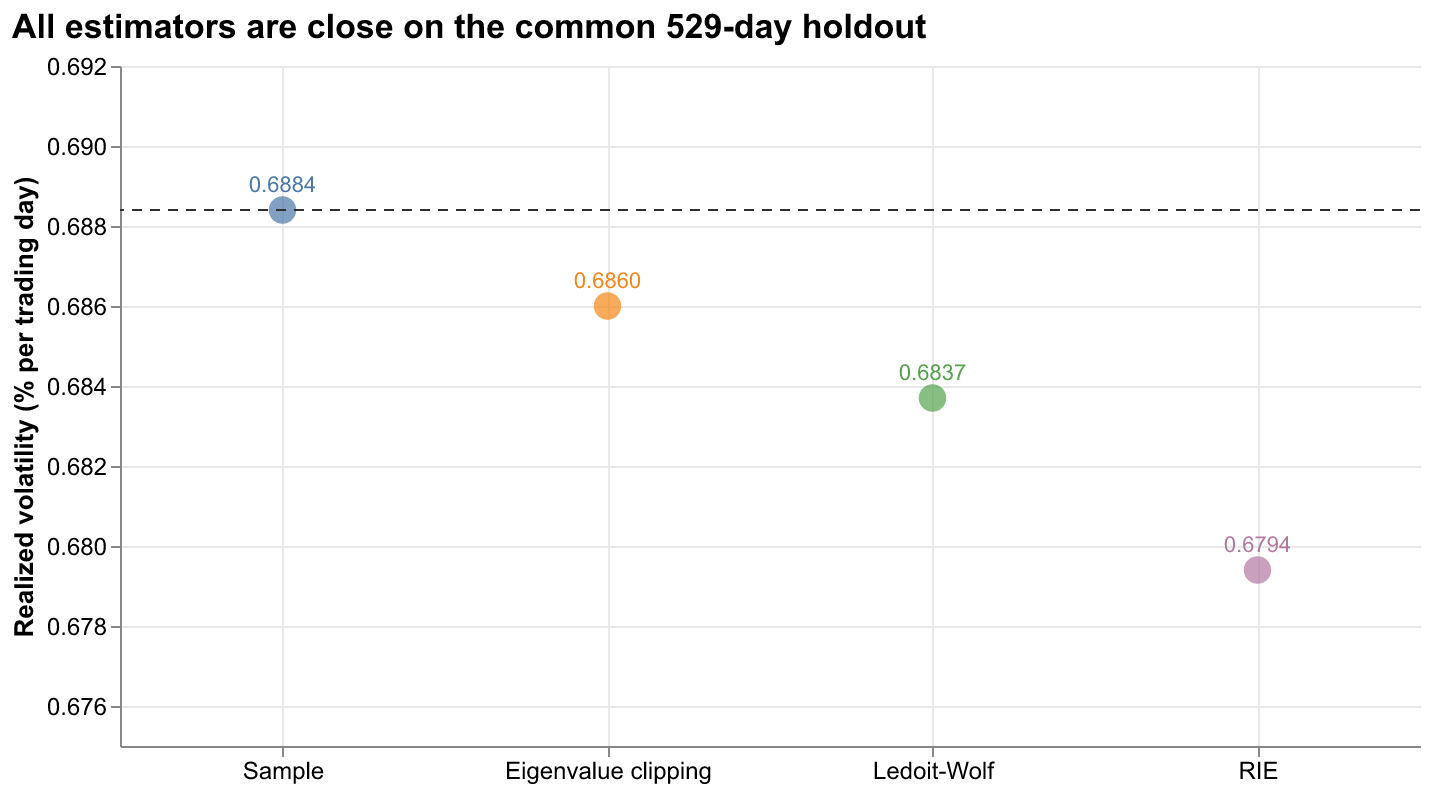
\includegraphics[width=0.88\textwidth]{../figures/figure1_primary_holdout.png}
\caption{Realized daily volatility on the common 529-day holdout. The dashed
line marks the sample-covariance estimate. The vertical axis is truncated to
show the small differences; this is a descriptive comparison and no
volatility-difference confidence interval is available.}
\label{fig:holdout}
\end{figure}

RIE's NEA is about 5.3\% higher than SM's on this split. The Shannon breadth
values, however, are almost identical (26.92 for both), and CL has a marginally
lower NEA but a slightly lower Shannon breadth. The conclusion is therefore
metric-dependent: spectral cleaning does not reduce either measure relative to
SM here, but the evidence for a practically large increase in diversity is
weak. This distinction is important when connecting portfolio concentration to
the broader concept of decision heterogeneity.

Figure~\ref{fig:breadth} puts both breadth statistics on separate scales.
RIE's higher NEA does not translate into a higher Shannon breadth, and
eigenvalue clipping has a lower NEA than SM. The defensible conclusion is
that RIE did not reduce either reported breadth measure relative to SM in
this sample, not that it produces a broad or diversified portfolio in an
absolute sense.

\begin{figure}[htbp]
\centering
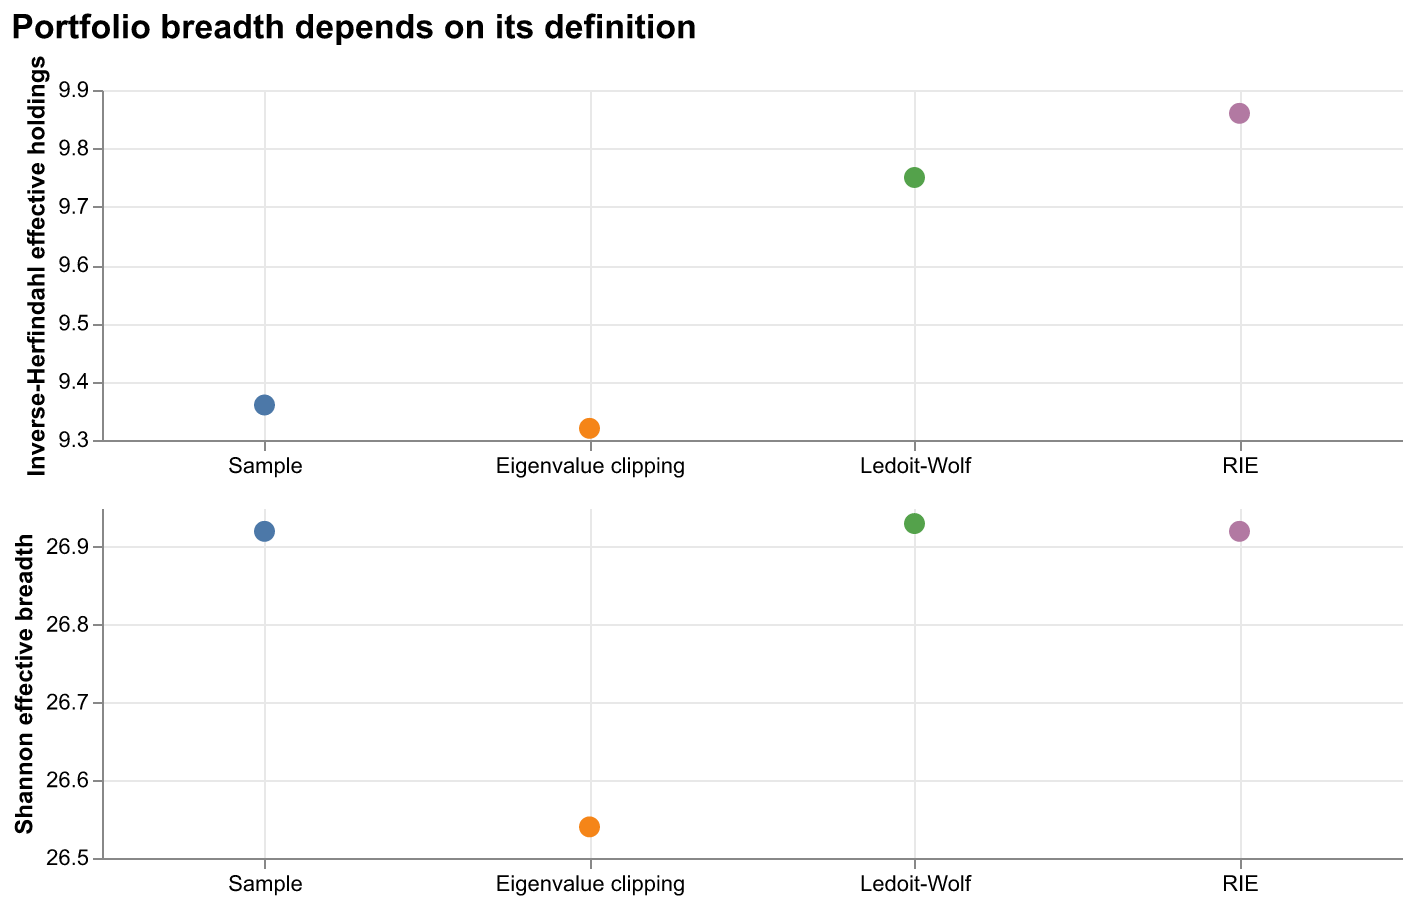
\includegraphics[width=0.88\textwidth]{../figures/figure2_allocation_breadth.png}
\caption{Two allocation-breadth summaries for the four optimized portfolios.
Each panel has its own vertical scale. Because short sales are allowed, these
statistics summarize weight concentration and are not literal counts of
long positions.}
\label{fig:breadth}
\end{figure}

The paired moving-block bootstrap, with 5,000 resamples and 20-day blocks, gives
an observed RIE--SM Sharpe difference of $+0.011$, a 95\% interval
$[-0.021,0.057]$, and one-sided $p=0.186$. We cannot reject equal Sharpe
performance on this holdout. The volatility difference is descriptive and is
not presented as a statistically significant treatment effect.

\subsection{Distributional sensitivity and market-regime validation}

In the rank-Gaussianized sensitivity, the ordering by holdout-to-training
volatility ratio remains CL, RIE, LW, SM; RIE does not rank first.
Table~\ref{tab:tails} gives the corresponding realized holdout volatilities.

\begin{table}[ht]
\centering
\caption{Holdout volatility under raw and rank-Gaussianized training marginals.
Evaluation always uses the same untransformed holdout returns.}
\label{tab:tails}
\small
\begin{tabular}{lrr}
\toprule
Estimator & Raw training returns & Rank-Gaussianized training returns \\
\midrule
SM & 0.6884 & 0.6942 \\
CL & 0.6860 & 0.6887 \\
LW & 0.6837 & 0.6919 \\
RIE & \textbf{0.6794} & \textbf{0.6870} \\
\bottomrule
\end{tabular}
\end{table}

For the primary training panel, per-asset excess kurtosis ranges from 1.18 to
20.20, with median 5.34, confirming substantial non-Gaussian tails. The
rank-Gaussianized sensitivity in Table~\ref{tab:tails} preserves the lower
holdout volatility of RIE relative to SM, but places CL first by the
holdout-to-training risk ratio. This robustness result is descriptive, and
does not establish that one estimator dominates under every distribution or
loss criterion.

Table~\ref{tab:vomregime} compares the same static portfolios on matched
holdout days above and below each converted VOM-series threshold. For
\texttt{VOMXCUS\$}, 188 matched days exceed the fixed training-period
90th-percentile threshold and 318 fall below it; realized portfolio
volatility is 30--32\% higher in the high state for all four estimators.
RIE's standard deviation is marginally lowest in both states. For
\texttt{VOMXGUS\$}, the high-state volatility increase is smaller and the
estimator differences are likewise modest. These conditional standard
deviations are descriptive rather than causal or inferential tests; the
Bloomberg export lacks field documentation needed to assign a definitive
economic interpretation to the VOM series. Figure~\ref{fig:regimes} shows
the full set of conditional standard deviations and makes clear that the
size of the high/low difference varies by proxy.

\begin{table}[ht]
\centering
\caption{Holdout daily portfolio volatility by converted VOM-series state
(percent per day). Thresholds are fixed at each series' training-period
90th percentile.}
\label{tab:vomregime}
\small
\begin{tabular}{llrrrrr}
\toprule
Proxy & State & Days & SM & CL & LW & RIE \\
\midrule
\texttt{VOMXCUS\$} & Below threshold & 318 & 0.6041 & 0.6033 & 0.5989 & 0.5961 \\
 & Above threshold & 188 & 0.7953 & 0.7873 & 0.7911 & 0.7845 \\
\texttt{VOMXGUS\$} & Below threshold & 333 & 0.6686 & 0.6719 & 0.6632 & 0.6594 \\
 & Above threshold & 173 & 0.7091 & 0.6905 & 0.7052 & 0.6998 \\
\bottomrule
\end{tabular}
\end{table}

\begin{figure}[htbp]
\centering
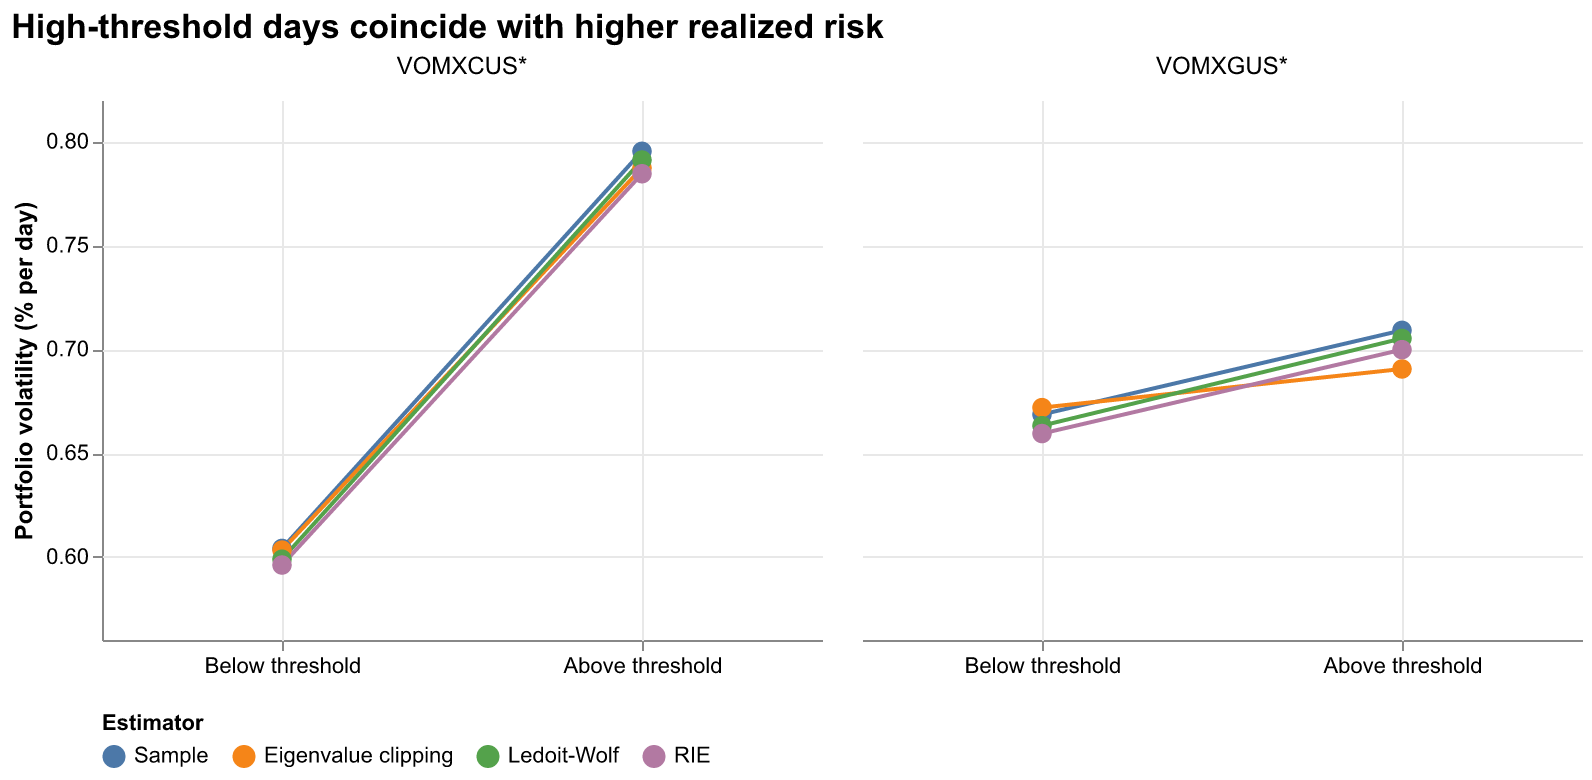
\includegraphics[width=0.96\textwidth]{../figures/figure3_market_regimes.png}
\caption{Holdout daily volatility conditional on the converted VOM-series
thresholds. Thresholds are estimated on the training period and held fixed;
no causal interpretation or regime-difference significance test is
available. Proxy field definitions remain unverified.}
\label{fig:regimes}
\end{figure}

\subsection{\texorpdfstring{Sensitivity to $q$}{Sensitivity to q}}

Recomputation from the matched 25-stock Bloomberg panel yields 100 daily
returns (13 May--29 September 2026), so $q=25/100=0.25$. Using the gross
total-return index, the sample covariance condition number is 279.55 and the
sample correlation condition number is 24.34. The largest sample-correlation
eigenvalue is 4.178, above the Marchenko--Pastur upper edge 2.25; one
eigenvalue lies above that edge. Eigenvalue clipping and diagonal
renormalization reduce the correlation condition number to 5.33 and the
covariance condition number to 128.49. Using unadjusted \texttt{PX\_LAST}
instead gives a correlation condition number of 24.31, a largest eigenvalue
of 4.170, and a clipped correlation condition number of 5.30. Clipping
reduces the correlation condition number by 78.1\% and the covariance
condition number by 54.0\%. The largest correlation eigenvalue, 4.178, is
1.86 times the random-matrix upper noise edge, with one eigenvalue above that
edge. This recent window illustrates spectral stabilization but has no
subsequent holdout, so improved conditioning cannot establish lower future
portfolio risk. These figures are recomputed from daily observations in the
latest workbook, not from reported summary statistics.

\begin{figure}[htbp]
\centering
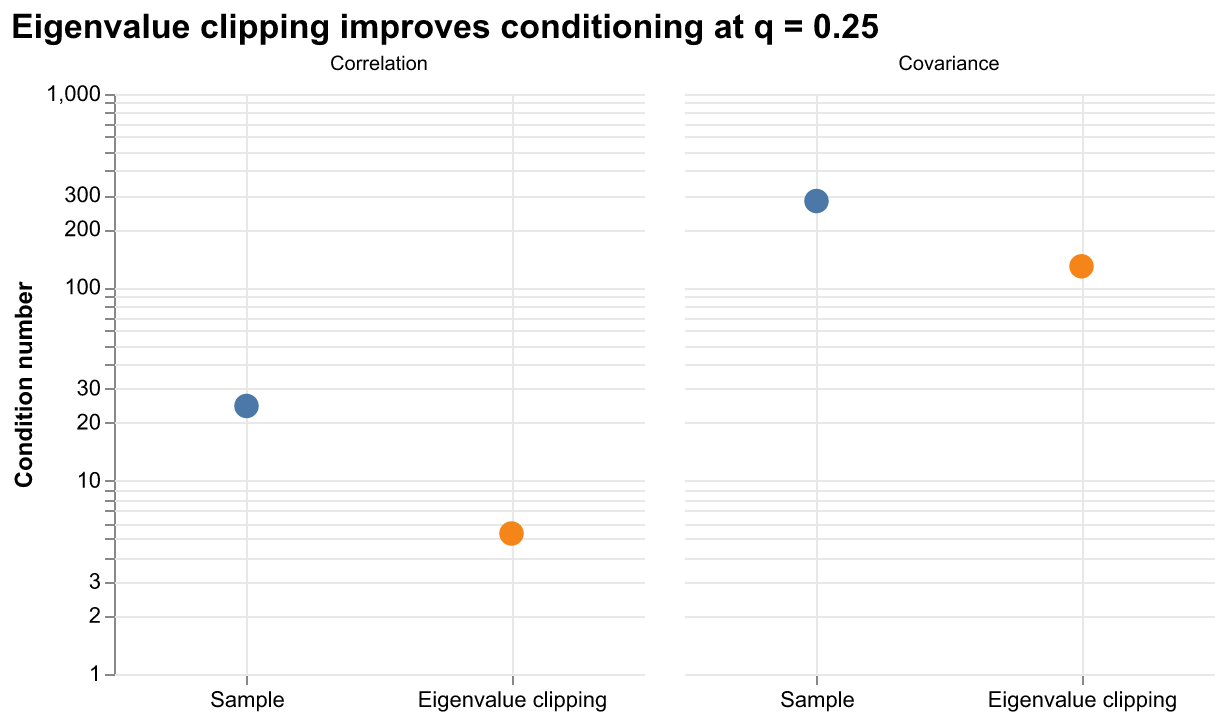
\includegraphics[width=0.88\textwidth]{../figures/figure4_conditioning.png}
\caption{Sample versus clipped condition numbers for covariance and
correlation matrices in the 25-stock gross-total-return panel
($q=0.25$; logarithmic vertical scale). Better conditioning is a numerical
property, not by itself an out-of-sample performance result.}
\label{fig:conditioning}
\end{figure}

At $q=1.9$ with 38 assets and 20 training days, the sample and unmodified RIE
covariance estimates are singular in all ten rolling windows and require a
pseudo-inverse. Across the following 60-day test windows, mean annualized
realized volatility is 16.57\% for SM, 11.78\% for CL, 12.12\% for LW, and
144.43\% for RIE (window-to-window standard deviation 320.17\% for RIE).
Thus the unmodified RIE implementation is unstable in this $q>1$ regime; no
extension to $q\geq1$ is claimed. Figure~\ref{fig:qgt1} uses a logarithmic
scale because the RIE mean is an order of magnitude larger than the other
three estimates. The exceptionally large 320.17\% between-window standard
deviation for RIE further indicates that its mean alone understates the
instability. The pseudo-inverse fallback makes these results a stress test of
the full pipeline, not a comparison of four equally well-posed estimators.

\begin{figure}[htbp]
\centering
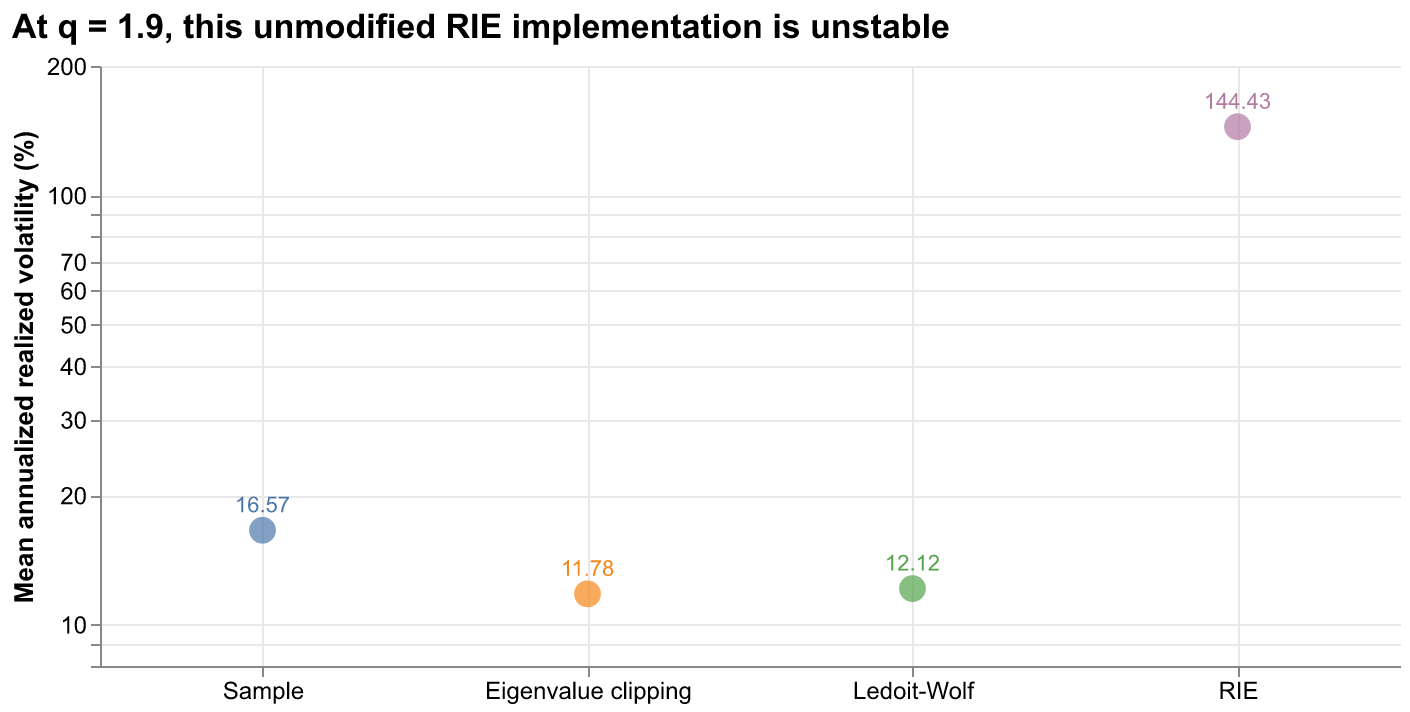
\includegraphics[width=0.88\textwidth]{../figures/figure5_q_gt_1.png}
\caption{Mean annualized realized volatility in ten deliberately short
$q=1.9$ training windows (logarithmic vertical scale). RIE's
window-to-window standard deviation is 320.17\%; the other estimators'
standard deviations were not preserved in the available output.}
\label{fig:qgt1}
\end{figure}

The distributional sensitivity in Table~\ref{tab:tails} is visualized in
Figure~\ref{fig:tails}. Training marginals are rank-Gaussianized and
rescaled, but evaluation remains on the unchanged holdout. RIE still has
lower holdout volatility than SM under this transformation; the result does
not hold against every alternative estimator, nor does it establish a
ranking by the holdout-to-training risk ratio.

\begin{figure}[htbp]
\centering
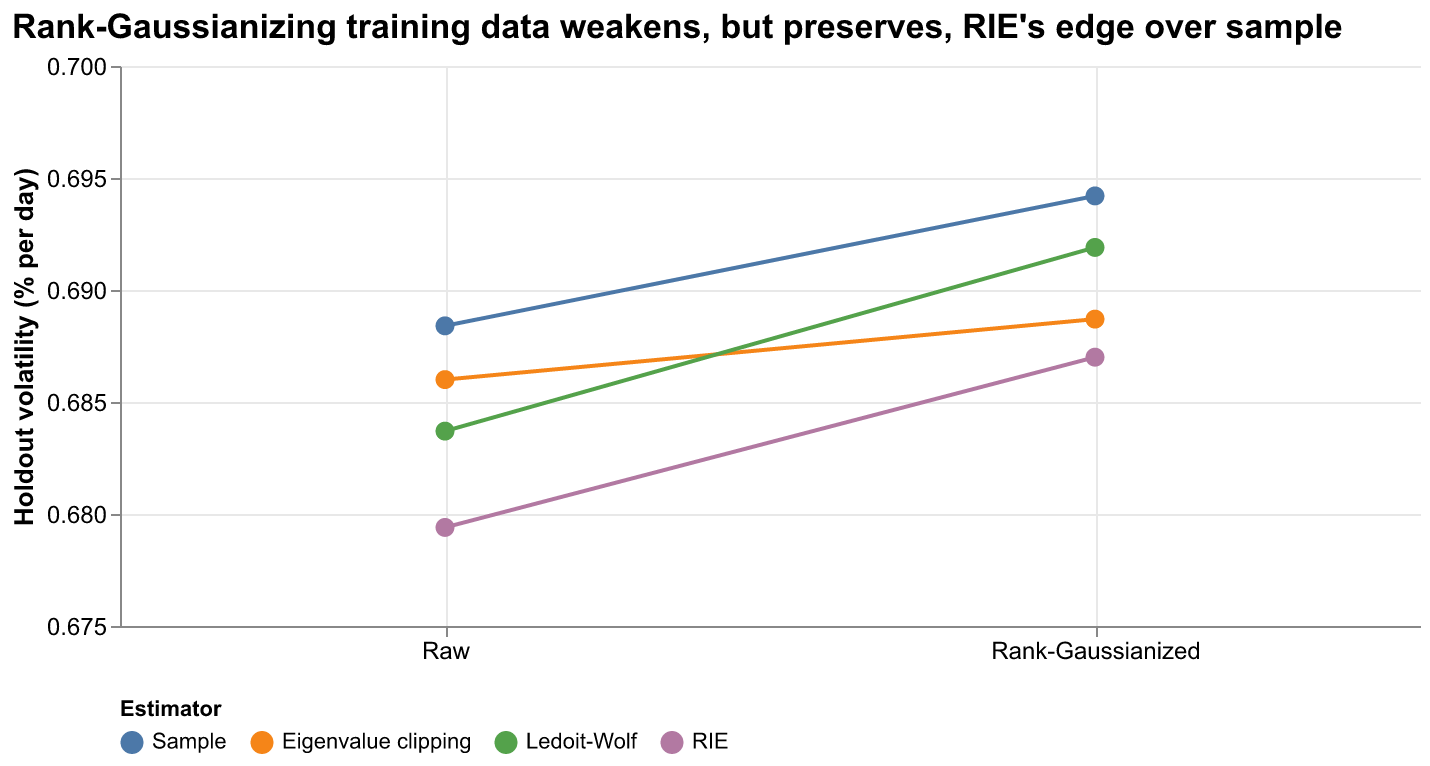
\includegraphics[width=0.88\textwidth]{../figures/figure6_distributional_robustness.png}
\caption{Holdout volatility after fitting on raw versus
rank-Gaussianized training marginals. The holdout is not transformed.
Truncated vertical scale highlights small differences.}
\label{fig:tails}
\end{figure}

\subsection{Fama--French factor check}
\label{sec:factor}

On the 522 holdout dates matched to the public daily Fama--French five-factor
file \cite{famafrench2015}, the RIE portfolio's estimated daily alpha is
0.000002 with $p=0.995$.
The other three estimators likewise have insignificant alphas ($p\geq0.887$).
This check does not support an abnormal-return claim. Because the factors are
constructed from U.S. equities while the test portfolios are Mexican, this
regression is an exploratory cross-market exposure diagnostic, not a
validated Mexican-equity pricing model. Its insignificant intercepts do not
establish factor neutrality.

\section{Discussion}

The primary answer is deliberately narrow. On one common BMV holdout, RIE
has the lowest point-estimate realized volatility, 1.31\% below SM in relative
terms, but the magnitude is small and the available bootstrap tests Sharpe
differences rather than volatility differences. Its Sharpe advantage over SM
is not statistically distinguishable from zero. This evidence is compatible
with a modest realized-risk improvement in this split; it does not establish
a general out-of-sample superiority of nonlinear shrinkage.

Allocation breadth also admits no unqualified "more diversified" conclusion.
RIE's inverse-Herfindahl count rises by 0.50 effective holdings (5.3\%) while
its Shannon breadth is unchanged at the reported precision. Moreover, the
weights are unconstrained and may be short, so these indices describe weight
concentration rather than literal portfolio membership. They do not measure
the diversity of investors, strategies, or beliefs in the market.

The regime comparisons are consistent with higher portfolio risk on
high-threshold VOM-labelled days, especially for VOMXCUS; the difference is
smaller for VOMXGUS. However, ticker semantics, data fields, and currency
interpretation are not documented in the export, and the exercise has no
reported uncertainty test. These results motivate validation of the proxy
metadata, not a claim that an identified economic regime causes a volatility
increase.

The $q=0.25$ cross-section shows that clipping can materially improve
numerical conditioning, including under a gross-total-return input. A better
condition number can reduce sensitivity of matrix inversion but does not
demonstrate improved realized risk by itself. Conversely, the $q=1.9$
experiment is a strong failure signal for this particular implementation:
unmodified RIE retains structural singularity and its realized-risk estimates
are extremely unstable. It is not a theorem about RIE in general, since the
kernel estimator and pseudo-inverse fallback were not redesigned for $q>1$.

Several limitations constrain external validity. First, the primary price
source is licensed, and the universe construction is not documented in enough
detail to rule out survivorship or selection bias. Second, one static
train/test split does not substitute for repeated rolling-origin evaluation;
no transaction costs, turnover, market impact, liquidity, short-sale
frictions, or leverage limits are modeled. Third, the assumed 8\% risk-free
rate is not varied, and no confidence interval for the volatility difference
is available. Fourth, the Bloomberg VOM definitions need independent
confirmation and the 25-stock recent panel is a fixed diagnostic set, not a
random sample of the 275-tab universe. Finally, the U.S. factor regression is
not a country-matched pricing test. The paper's conclusion should therefore
be read as evidence about a particular panel, split, implementation, and
portfolio construction.

\section{Conclusion}

For the common 38-stock BMV holdout, nonlinear spectral cleaning is associated
with a small reduction in realized minimum-variance risk and no measured
reduction in either reported allocation-breadth measure relative to the
sample estimator. The Sharpe-ratio difference is not statistically
significant, and Shannon breadth is unchanged. The supplementary evidence
shows descriptive regime dependence, numerical conditioning gains at
$q=0.25$, and a severe instability boundary for the unmodified RIE
implementation at $q=1.9$. The evidence supports considering RIE as one
covariance-estimation option in the low-$q$ setting studied, with repeated
out-of-sample monitoring and explicit estimator-validity checks. It does not
establish universal estimator dominance or market-wide changes in investor
heterogeneity.

\paragraph{Data availability.}
The Fama--French five-factor series is available from the Kenneth French Data
Library (\url{https://mba.tuck.dartmouth.edu/pages/faculty/ken.french/data_library.html}).
The primary Econom\'atica prices and supplementary Bloomberg exports
(the VOM/NAFTRAC/USD--MXN CSV and the 275-instrument BMV/BIVA workbook,
downloaded in September 2026) are subject to data-provider terms and are not
included. This working paper's companion repository
(\url{https://github.com/IvliCaesar/bmv-spectral-portfolio-cleaning})
contains only aggregate
summary tables and charts, not daily prices, returns, security weights, or
licensed exports. Those summary outputs allow readers to recreate the
displayed graphics and check selected arithmetic; they do not permit
re-estimation of the portfolios, bootstrap, factor regressions, regime
classification, or eigenspectra. The companion repository does not include
the original estimator-analysis scripts; full replication therefore requires
lawful access to both licensed inputs and the complete analysis workflow.

\begin{thebibliography}{9}
\small

\bibitem{markowitz1952}
H. Markowitz, Portfolio selection, \textit{The Journal of Finance} 7 (1952),
no.~1, 77--91.

\bibitem{marchenko1967}
V.~A. Marchenko and L.~A. Pastur, Distribution of eigenvalues for some sets of
random matrices, \textit{Mathematics of the USSR-Sbornik} 1 (1967), no.~4,
457--483.

\bibitem{laloux1999}
L. Laloux, P. Cizeau, J.-P. Bouchaud, and M. Potters, Noise dressing of
financial correlation matrices, \textit{Physical Review Letters} 83 (1999),
no.~7, 1467--1470.

\bibitem{pafka2002}
S. Pafka and I. Kondor, Noisy covariance matrices and portfolio optimization,
\textit{The European Physical Journal B} 27 (2002), 277--280.

\bibitem{ledoitwolf2004}
O. Ledoit and M. Wolf, Honey, I shrunk the sample covariance matrix,
\textit{The Journal of Portfolio Management} 30 (2004), no.~4, 110--119.

\bibitem{ledoit2022}
O. Ledoit and M. Wolf, Analytical nonlinear shrinkage of large-dimensional
covariance matrices, \textit{The Annals of Statistics} 50 (2022), no.~6,
3791--3816.

\bibitem{demiguel2009}
V. DeMiguel, L. Garlappi, and R. Uppal, Optimal versus naive diversification:
how inefficient is the $1/N$ portfolio strategy?, \textit{The Review of
Financial Studies} 22 (2009), no.~5, 1915--1953.

\bibitem{famafrench2015}
E.~F. Fama and K.~R. French, A five-factor asset pricing model,
\textit{Journal of Financial Economics} 116 (2015), no.~1, 1--22.

\end{thebibliography}

\end{document}
